\documentclass[type = bachelor, oneside]{whu-thesis}
\usepackage{textcomp,mathcomp}
\usepackage{siunitx}
\usepackage{chemfig}
\usepackage{graphicx}

\whusetup
  {
    info               =
      {
        title          = {金刚石氮-空位色心的\\电荷态调控和性质表征},
        title*         = {Modulation of Charge States and Characterization of Properties\\ in Nitrogen-Vacancy Centers of Diamond},
        student-number = {2020302192129},
        school         = {弘毅学堂},
        author         = {邹迪玮},
        author*        = {Diwei Zou},
        subject        = {学科},
        major          = {微电子科学与工程},
        advisor        = {周利 , 副教授;孙启超 , 研究员},
        direction      = {研究方向},
        date           = {2024/5},
        keywords       = {关键词 1 , 关键词 2 , 关键词 3 , 关键词 4 , 一个非常非常,非常非常长——的关键词 5},
        keywords*      = {key word 1 , key word 2 , key word 3 , key word 4 , {and a very very, very very long key word---the key word 5}},
      },
    style              =
      {
        graphics-path  = {{figures/}{data/}},
        list-of-figures,
        list-of-tables,
      },
    element            =
      {
        innovation     = {pages/innovation},
        abstract       = {pages/abstract},
        abstract*      = {pages/enabstract},
        bibliography   = {ref/refs_all}
      }
  }
\begin{document}

% Chapter 1

\chapter{绪论}

\section{研究背景}
互联网已经成为我们日常生活中不可或缺的一部分。自1969年实现第一个互联网原型以来的短短50年间,全球网络已经融入了我们日常生活的方方面面。我们通过电子邮件和社交媒体进行交流,在线阅读新闻,使用在线导航工具规划交通路线,通过在线商店订购杂货或服装,甚至可以在线安排所有的金融事务 \cite{Internet2024Wiley}。

同经典互联网带来许多意想不到的应用一样,未来的量子互联网(Quantum Network)也将带来革命性的成果和应用。在量子互联网中,信息将使用量子比特(Quantum bit,Qubit)来进行描述和传递,这些qubit遵循量子力学的规则,因此表现出不同于它们的经典对应物的行为,特别是创建叠加态(Superposition state)和纠缠态(Entanglement state)的可能性,以及执行投影测量(Project Measurement)等特征,赋予了量子互联网其独特的优势。已经知道了未来量子互联网的几种有前景的应用,比如墨子号实现的量子保密安全通信,在云端进行具有完全隐私性的量子计算,以及量子精密测量等等 \cite{Ekert2014,Jiang2007,Broadbent2009,Gottesman2012,Nickerson2014,Komar2014}。此外,量子互联网甚至可以作为测试量子力学本身的平台,来对未来的各种应用进行可能的探究,拥有者较为广阔的应用前景 \cite{Hensen2015, Wehner2018}。

对于构建量子网络而言,需要选择特定的体系来构建量子比特。目前,已经有许多种量子比特的实现方案,比如超导量子比特(Superconducting Qubit)、离子阱量子比特(Ion Trap Qubit)、硅基量子比特(Silicon Qubit)等等。其中,金刚石中的氮-空位色心(Nitrogen-Vacancy Center,NV Center)由于其长寿命、稳定性、易于操控等特点,被广泛应用于量子信息科学中。NV Center是一种由金刚石晶格中的氮原子取代碳原子和空位形成的缺陷,其电子能级结构具有多个电子态,可以被激光激发和退激发,发射的荧光光子可以被探测器接收,从而实现对NV Center的探测和成像。NV Center的电子态可以被微波和射频场调控,实现对NV Center的操控和量子态的制备,是构建量子网络的重要组成部分 \cite{Doherty2013,Childress2014}。

在过去的研究中,通过精准的相位锁定、快速的自旋操作等高端技术,NV Center表现出了优异的性能。近些年来,荷兰代尔夫特理工大学的QuTech公司的$R.Hanson$的团队在2021年实现了实验室级别的多节点量子网络,通过NV Center实现了两个量子比特之间的量子隐态传输(Quantum Teleportation),如图 \ref{fig: Remote Entanglement}(a)所示 \cite{Pompili2021}。
\begin{figure}
  \centering
  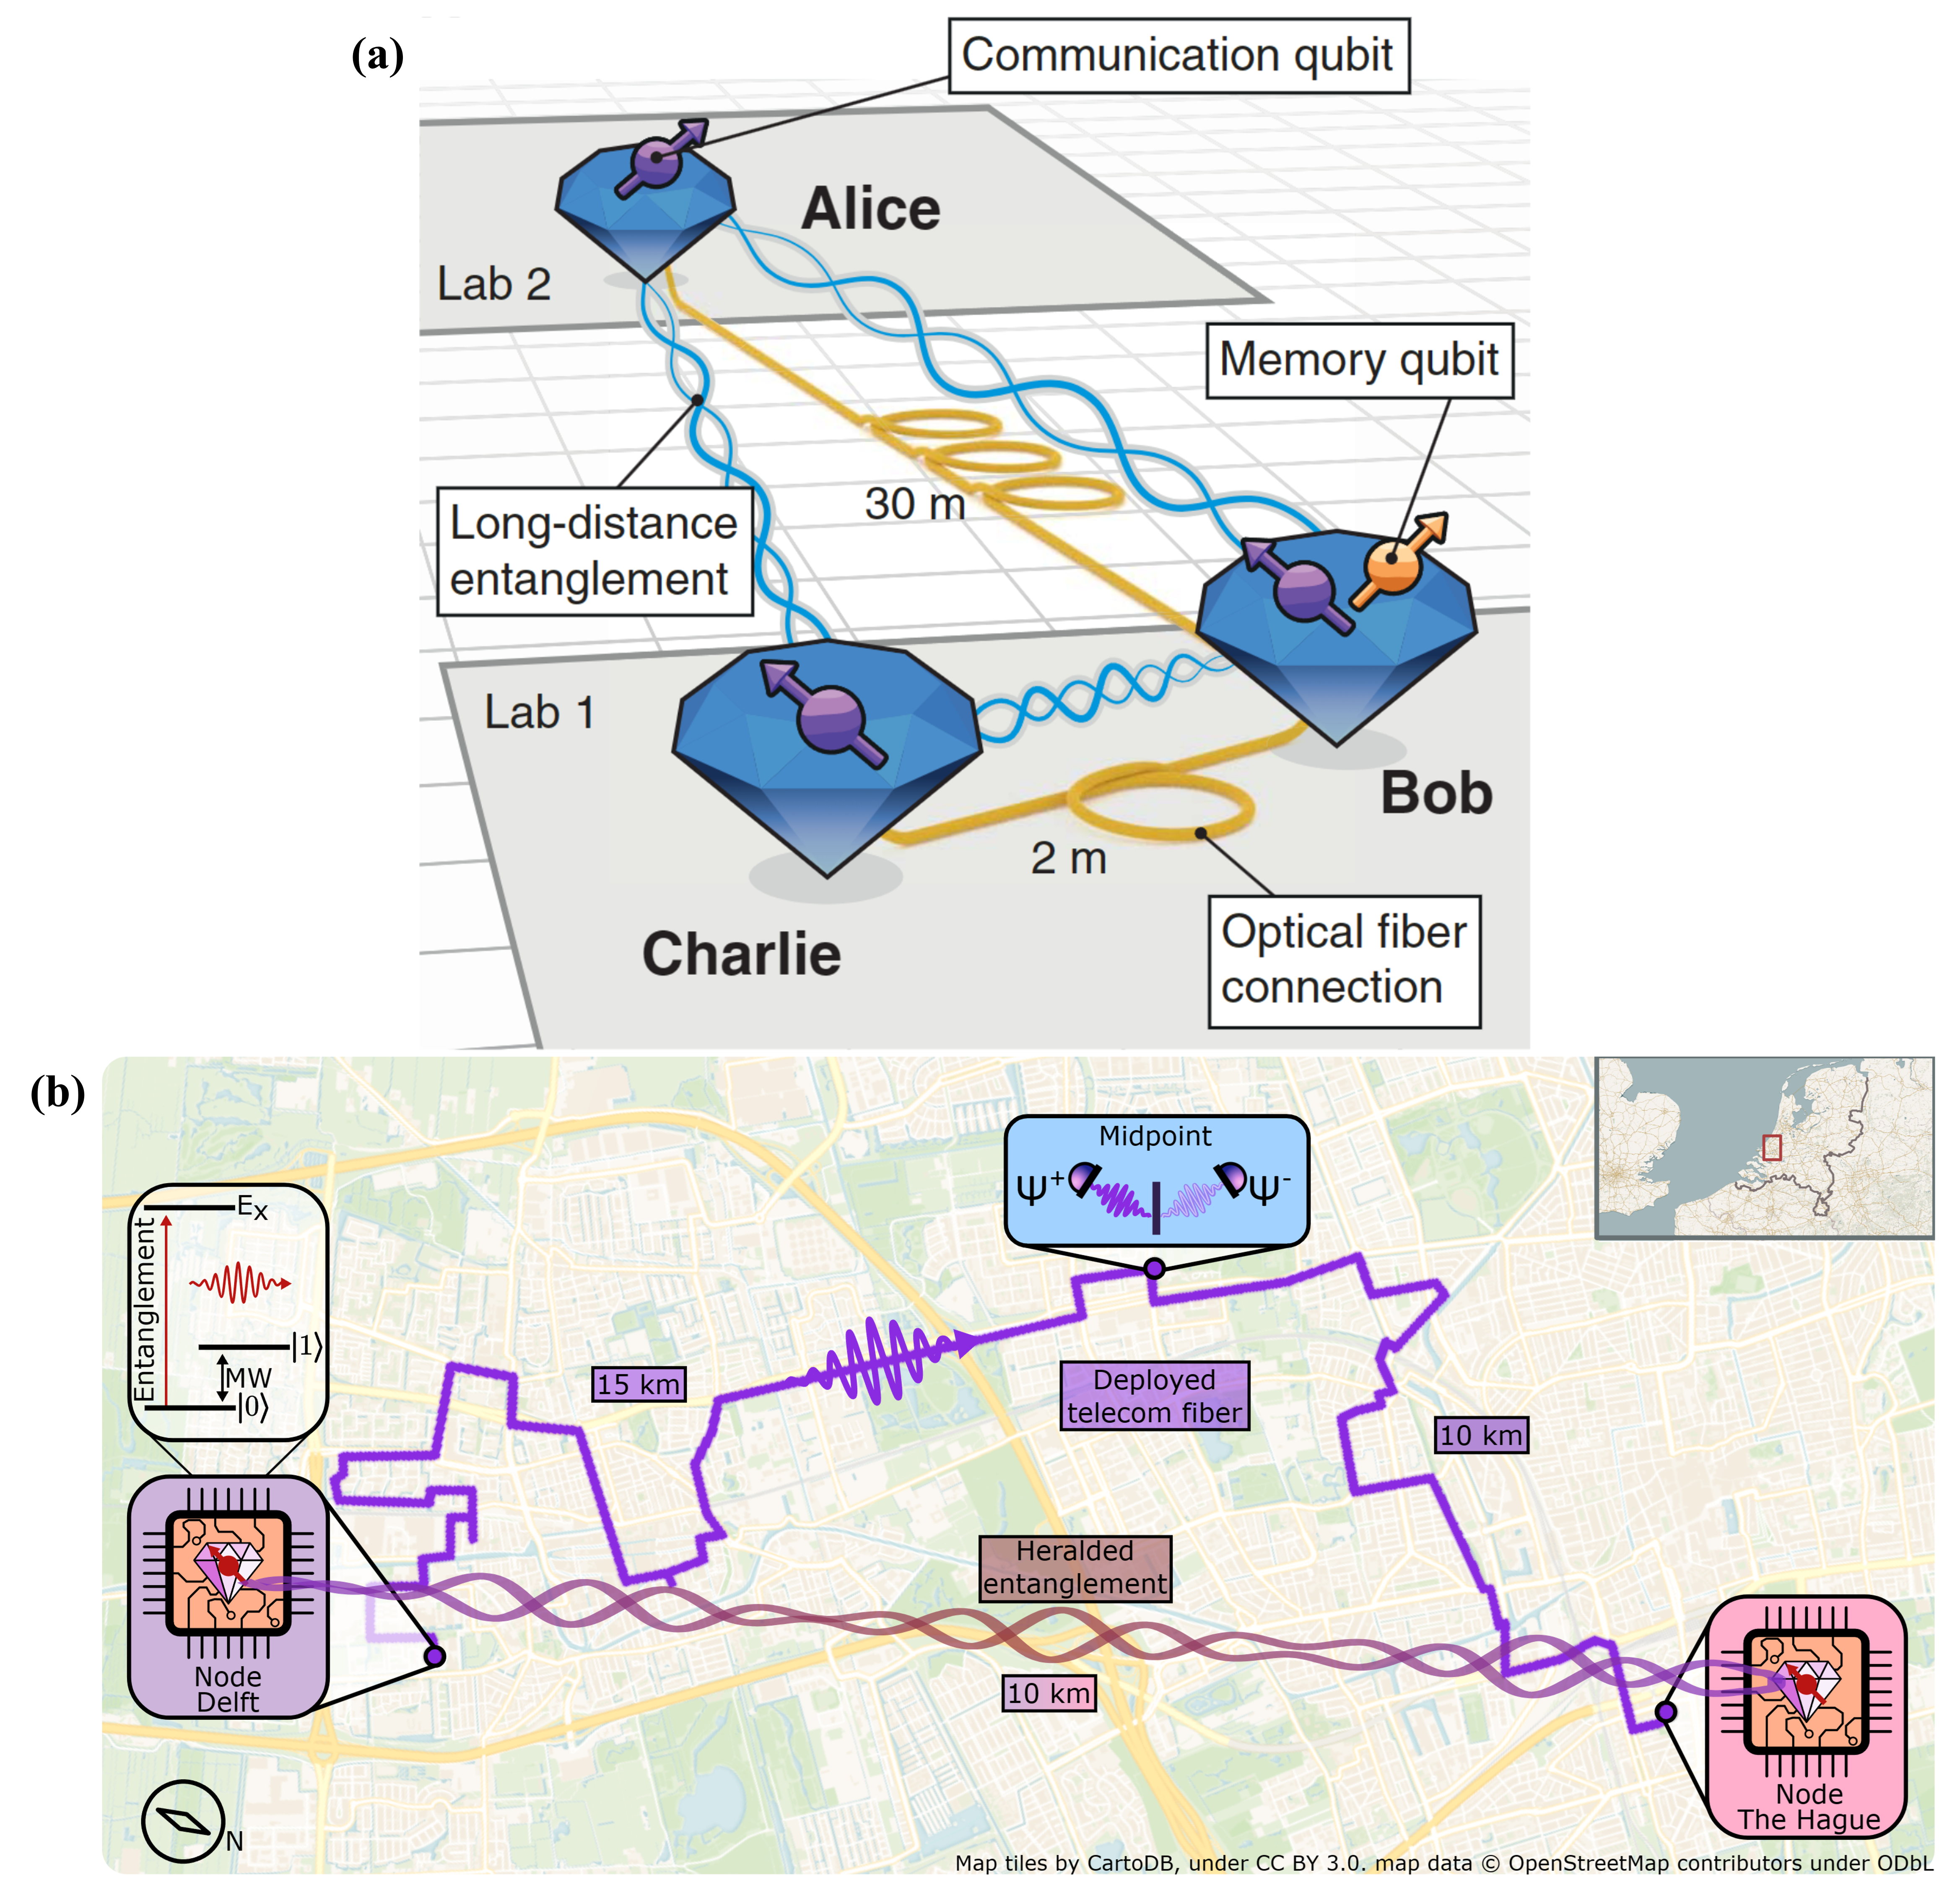
\includegraphics[width=1.0\textwidth]{figures/Chapter 1/Remote Entanglement.png}
  \caption[NV Center构建的量子网络]{NV Center构建的量子网络,(a)实现了实验室距离尺度的Quantum Teleportation,(b)实现城际尺度的QUantum Entanglement \cite{Pompili2021,Stolk2024}。}
  \label{fig: Remote Entanglement}
\end{figure}
最近,其团队利用NV Center实现城际尺度的Quantum Entanglement,如图 \ref{fig: Remote Entanglement}(a)所示,表明NV Center作为量子比特的潜力巨大,为未来量子网络的构建提供了重要的参考 \cite{Stolk2024}。

\section{研究目的和意义}

一般来说,我们在利用NV Center作为Qubit的时候,是利用其电子自旋和核自旋所携带的自旋状态信息作为信息载体,然而NV Center的电荷态同样可以作为一种信息的载体进行操控、传递和读出。通常情况下,由于NV Center的能级结构和电子分布的特性,绝大部分时候的NV Center都是处于负电中心的状态,即为NV$^-$的状态,这个时候自旋量子数$S=1$,其能被532 nm的激光激发,在退激发的过程中释放出637 nm的零声子线和波长更长的声子边带,通过记录发射的光子来读出NV Center的电子自旋信息。然而在特定的情况下,受到外界环境的影响和激光的错误激发,NV Center中可能会存在中性的电荷态即NV$^0$,即使是对于单个的NV Center而言,NV$^-$和NV$^-$可能同时存在,并处于一个动态平衡相互转化的过程 \cite{Shields2015,Hacquebard2018,Shinei2021}。在前人的研究中,其最重要的理论依据是NV Center的自旋状态也可以通过映射到电荷态进行读出,因此NV Center的电荷态可以用于许多比较特殊的用途,比如在电场感应进行相干性控制和对电场进行精密测量等方面,已经取得了较为明显的进展 \cite{Yan2022,Kurokawa2023}。

在很多时候,我们需要判断某一个发光的亮点是否为单个NV Center,从而对其进行单自旋调控,这个时候通常是利用其二阶关联函数进行判断,如图 \ref{fig: g2_function}所示,最低点低于0.5的时候,即可认为该点为单个的NV Center \cite{Sow2020,Robledo2011,Doherty2012}。
\begin{figure}
  \centering
  \includegraphics[width=0.8 \textwidth]{figures/Chapter 1/g2_function.png}
  \caption[NV Center的二阶关联函数]{NV Center的二阶关联函数 \cite{Sow2020}。}
  \label{fig: g2_function}
\end{figure}
而通过观测NV Center的电荷态分布,给了我们另一种判断是否为单个NV Center的依据,即如果存在两个及以上的NV Center的话,不止一个的NV Center的电荷态会存在多种概率分布的曲线,叠加到一起后会出现不止两个峰值。所以基于这个原理,提供了一种新的检测思路,NV Center的电荷态表征也能在仅有一个单光子计数器的情况下,对多个NV Center的位点进行判断和排除,而不必依赖于两个单光子计数器

除此之外,由于我们在利用NV Center作为量子信息的载体的过程中,主要是利用其NV$^-$的自旋量子数$S=1$的特性对电子自旋进行精准的调控,因此我们希望NV Center尽可能多的处于NV$^-$的状态下,所以对与NV Center电荷态的调控和性质表征就尤为重要,尤其是在进行量子门操作的时候,对电荷态的分布规律进行观测,从而进行电荷态共振检查(Charge Resonance Check,CRC),以确保在进行量子纠缠、量子隐态传输、量子蒸馏提纯等操作过程中的保真度,提高量子通信网络的稳定性和准确性。

\section{论文结构}

本文的工作主要是基于金刚石NV Center的电荷态调控和性质表征,在第一章绪论中介绍了NV Center作为量子比特构建量子网络和其电荷态在实际实验中的意义和应用。随后,在第二章详细介绍了金刚石中的NV Center这一体系的性质,包括宏观层面的外观、形态、制备方法,微观层面的晶体结构、原子组成、电子能级、光学和自选性质等,以及量子层面的哈密顿量、相干性质和自选调控的操作。进一步地,在第三章中,结合我们的目标和预期结果,构建NV Center电荷态动力学的理论模型及相关的公式推导。然后在第四章中介绍了实验的平台搭建过程和细节,以及测量的序列设置和数据的后处理方案。紧接着就通过理论仿真和实验数据观测了NV Center的电荷态分布情况,讨论了NV$^-$和NV$^0$的计数率和相互之间的转化效率在不同的实验条件下的变化。最后,对全文进行了总结和对未来的展望。
 
\end{document}